\problemname{Meddelande}
\noindent
I staden som Paula bor i finns ett stort torg. Torget kan representeras av ett 
rutnät med $N$ rader och $M$ kolumner. I vissa av rutorna finns det bokstäver 
inristade. 

Enligt legenden så bildar dessa bokstäver ett meddelande om man 
går på rutorna i en viss ordning. För att det ska bli rätt måste man börja 
i det övre vänstra hörnet och sluta i det nedre högra hörnet, och man får bara gå steg åt höger 
och nedåt. Om man lyckas besöka alla bokstavsrutorna på det här viset så bildas 
det hemliga meddelandet. 

Paula har beslutat sig för att en gång för alla knäcka gåtan, och hitta meddelandet.

Skriv ett program som hittar meddelandet, givet rutnätet.

\section*{Indata}
Den första raden innehåller två heltal $N$ och $M$ ($1 \leq N,M \leq 6$), 
antalet rader och kolumner i rutnätet.

Följande $N$ rader innehåller en sträng av längd $M$ vardera. Dessa strängar 
representerar raderna i rutnätet, och innehåller små bokstäver \texttt{a}-\texttt{z} och punkter ``.''.
Punkterna representerar tomma rutor.

Det är garanterat att det går att besöka alla rutorna med bokstäver genom att 
starta i det övre vänstra hörnet och gå höger och nedåt till det nedre högra hörnet.

\section*{Utdata}
Skriv ut en sträng, det hemliga meddelandet.

\section*{Poängsättning}
Din lösning kommer att testas på en mängd testfallsgrupper.
För att få poäng för en grupp så måste du klara alla testfall i gruppen.

\noindent
\begin{tabular}{| l | l | p{12cm} |}
  \hline
  \textbf{Grupp} & \textbf{Poäng} & \textbf{Gränser} \\ \hline
  $1$    & $20$       & $N = 1$ \\ \hline
  $2$    & $40$       & Antalet bokstäver är $N+M-1$. \\ \hline
  $3$    & $40$       & Inga ytterligare begränsningar. \\ \hline
\end{tabular}

\section*{Förklaring av exempelfall 1}

\begin{figure}[h]
  \centering
  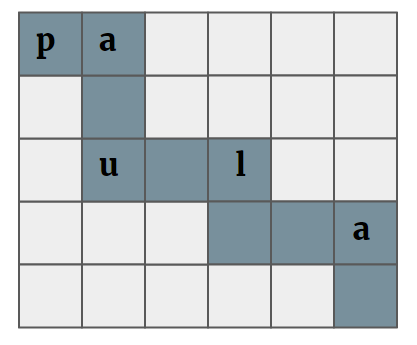
\includegraphics[width=0.3\textwidth]{sample.PNG}
    \\Bilden visar lösningen till exempelfall 1. De mörka rutorna visar ett möjligt
    sätt att gå från övre vänstra hörnet till nedre högra hörnet, så att alla 
    bokstäver besöks.
  
\end{figure}
